\documentclass{emulateapj}
%\documentclass[12pt,preprint]{aastex}

\usepackage{graphicx}
\usepackage{float}
\usepackage{amsmath}
\usepackage{epsfig,floatflt}
\usepackage{url}
\usepackage{subfig}
\setcitestyle{square}




\begin{document}

\title{Project 4}

\author{Christer Dreierstad}

\email{chrisdre@student.matnat.uio.no}

\altaffiltext{1}{Institute of Physics, University of
  Oslo, P.O.\ Box 1029 Blindern, N-0315 Oslo, Norway}


%\date{Received - / Accepted -}

\begin{abstract}

\end{abstract}
\keywords{computational science: Ising model  --- methods: Metropolis, Monte Carlo}

\section{Introduction}
\label{sec:introduction}
To study the phase transitions of a magnetic system we consider the Ising model for a two-dimensional system with a finite lattice size. The particles (spins) that make up the crystal (lattice) can take two values representing spin up or down. The energy of the lattice can then, by the Ising model, be found by
%
\begin{gather}\label{eq:energyIsing}
    E = -J\sum_{< kl >}^N s_k s_l,
\end{gather}
%
when there is no external magnetic field applied to the system. The coupling constant J will be set to 1, which means we are studying a ferromagnetic interaction between the spins that make up the lattice. Since the coupling constant is dependent upon the material we study, setting this to 1 allows for a general model. For studying the phase transition we use a Markov chain Monte Carlo method (MCMC), and the probability of finding the system in a given state $i$ is
%
\begin{align*}
    P(E_i) = \frac{e^{-\beta E_i}}{Z},
\end{align*}
%
where Z is the partition function $Z = \sum_i e^{-\beta E_i}$, which is impossible to calculate unless we know all the states. To eliminate the partition function we will use the Metropolis algorithm, which eliminates the partition function. When applying the algorithm we will consider periodic boundary conditions of the lattice, which will allow us to simulate an infinitely large lattice, and we do not have to consider what happens on the boundary the lattice (the ends of the material). Increasing the size of the lattice will further improve the approximation of a large scale lattice. The goal of the MCMC simulation is to observe the energy and the magnetic moment as time (MC cycles) increase, we expect the system to stabilize in the most probable state.


\section{Method}
\subsection{Analytical expressions}
\label{sec:method}
\begin{deluxetable}{cccc}
\tablewidth{0pt}
\tablecaption{\label{tab:energies}}
\tablecomments{States of the 2x2 lattice and corresponding values for energy and magnetic moment. Notice that the ground state (the lowest energy) has either all spins pointing up or down.}
\tablecolumns{4}
\tablehead{Spins up  & Degeneracy & Energy & Magnetic moment}
\startdata
4 & 1 & -8J & 4 \\
3 & 4 & 0 & 2 \\
2 & 4 & 0 & 0 \\
2 & 2 & 8J & 0 \\
1 & 4 & 0 & -2 \\
0 & 1 & -8J & -4
\enddata
\end{deluxetable}

The two-dimensional binary Ising model has analytical expectation values. The partition function
%
\begin{equation*}
    z = \sum_i \Omega(E_i) e^{\beta E_i},
\end{equation*}
%
where $\Omega(E_i)$ is the degeneracy of energy $E_i$ and $\beta = 1/k_BT$. From Table \ref{tab:energies} we can see that there are 2 energies that are non-zero: $\pm 8J$, which both has a degeneracy of 2. The energy equal to zero has a degeneracy of 12. Expanding the sum of the partition function we get 
%
\begin{align*}
    z &= 2e^{8J\beta} + 12 + 2e^{-8J\beta} \\
    &= 12 + 2\left(e^{8J\beta} + e^{-8J\beta}\right),
\end{align*}
%
where we have inserted $e^0 = 1$. We know that $\cosh(x) = \frac{1}{2}\left( e^{-x} + e^x\right)$, inserting this gives
%
\begin{gather}\label{eq:z}
    Z = 12 + 4\cosh(8J\beta).
\end{gather}
%
The mean value of the energy is given by
%
\begin{align*}
    \langle E \rangle = -\frac{\partial }{\partial \beta} \ln Z = -\frac{1}{Z}\frac{\partial Z}{\partial \beta},
\end{align*}
%
which is found by inserting the partition function.
%
\begin{align*}
    \langle E \rangle &= -\frac{1}{Z}\frac{\partial}{\partial \beta} \left(12 + 4 \cosh\left(8J\beta\right)\right)\\
    &= -\frac{4}{Z}\left(8J\sinh\left(8J\beta\right)\right),
\end{align*}
pulling a factor 4 from the partition function and inserting we are left with a analytical solution to the mean energy of the lattice
%
\begin{gather*}
    \langle E \rangle = -\frac{8J\sinh\left(8J\beta\right)}{3 + \cosh(8J\beta}.
\end{gather*}
%
The heat capacity can be found by
%
\begin{align*}
    C_V &= \frac{1}{kT^2}\frac{\partial^2}{\partial \beta^2} \ln Z = \frac{1}{kT^2}\frac{\partial}{\partial \beta}\left(\frac{\partial}{\partial \beta} \ln Z\right),
\end{align*}
%
where we recognize the partial derivative in the parenthesis as the negative mean energy. 
%
\begin{align*}
    C_V = \frac{1}{kT^2}&\left(\frac{64J^2\cosh\left(8J\beta\right)\left(3 + \cosh\left(8J\beta\right)\right)}{\left(3 + \cosh\left(8J\beta\right)\right)^2}\right \\
    &-\left \frac{64J^2\sinh^2\left(8J\beta\right)}{\left(3 + \cosh\left(8J\beta\right)\right)^2}\right),
\end{align*}
%
by inserting for the mean energy and using the product rule. Further simplifications gives the mean heat capacity
%
\begin{gather*}
    C_V = \frac{64J^2}{k_B T^2} \left(\frac{\cosh(8\beta J)(3+\cosh(8 \beta J)) - \sinh^2(8\beta J)}{\left(3 + \cosh(8\beta J)\right)^2}\right)
\end{gather*}
The susceptibility is given as
%
\begin{equation*}
    \chi = \frac{1}{kT}\left(\langle M^2 \rangle - \langle M \rangle^2\right).
\end{equation*}
%
To find the susceptibility of the system we consider the mean magnetic moment
%
\begin{equation*}
    \langle M \rangle = \frac{1}{Z} \sum_i |M_i| e^{-\beta E_i},
\end{equation*}
where we find the magnetic moment for a given energy in Table \ref{tab:energies}. So the mean magnetic moment is
%
\begin{equation*}
    \langle M \rangle = \frac{1}{Z}\left(4e^{8J\beta} + 4\left(2e^{0}\right) + 4\left(-2e^0\right) + -4e^{8J\beta} \right) = 0.
\end{equation*}
%
Further we calculate the mean of the  magnetic moment squared
%
\begin{equation*}
    \langle M^2 \rangle = \frac{1}{Z}\sum_i M_i^2 e^{-\beta E_i},
\end{equation*}
and again referring to Table \ref{tab:energies} we get
%
\begin{align*}
    \langle M^2 \rangle &= \frac{1}{Z}\left(16\left(2e^{8J\beta}\right) + 16\left(2e^0\right) \right) \\
    &= \frac{8\left(e^{8J\beta} + 1\right)}{3 + \cosh\left(8J\beta\right)}.
\end{align*}
So the susceptibility of the system is given as
%
\begin{equation*}
    \chi = \frac{1}{kT^2}\langle M^2 \rangle = \frac{1}{kT^2}\frac{8\left(e^{8J\beta} + 1\right)}{3 + \cosh\left(8J\beta\right)}
\end{equation*}
%
Further we find the mean of the absolute value of the magnetic moment by

\begin{align*}
    \langle |M| \rangle &= \frac{1}{Z} \sum_i |M_i| e^{-\beta E_i} \\
     &= \frac{1}{Z}\left(4e^{8J\beta} + 4\left(2e^{0}\right) + 4\left(|-2|e^0\right) + |-4|e^{8J\beta} \right) \\
     &= \frac{2e^{8J\beta} + 4}{3 + \cosh\left(8J\beta\right)},
\end{align*}
%
after pulling out a factor 4 from the partition function. To summarize we have the following analytical expression for the system
%
\begin{align*}
    &\langle E \rangle = -\frac{4}{Z}\left(8J\sinh\left(8J\beta\right)\right), \\
    &\langle |M| \rangle = \frac{2e^{8J\beta} + 4}{3 + \cosh\left(8J\beta\right)}, \\
    &C_V = \frac{64J^2}{k T^2} \left(\frac{\cosh(8\beta J)(3+\cosh(8 \beta J)) - \sinh^2(8\beta J)}{\left(3 + \cosh(8\beta J)\right)^2}\right), \\
    &\chi = \frac{1}{kT^2}\frac{8\left(e^{8J\beta} + 1\right)}{3 + \cosh\left(8J\beta\right)}.
\end{align*}

\subsection{Ising model}
When the energy of the Ising model we consider the equation given in the introduction, Eq. \eqref{eq:energyIsing}, where the subscript of the sum means we are taking the sum over the neighbouring spins, N is the total amount of spins and $s_k$, $s_l = \pm 1$, represents the spin of the particles. Consider a random spin at the lattice, in the two-dimensional case it has a total of four neighbours that it interacts with.  An example for a spin surrounded by four spin up.
%
\begin{equation*}
    \begin{matrix}
    & \uparrow & \\
    \uparrow & \uparrow & \uparrow \\
    & \uparrow & \\
    \end{matrix},
   % \quad
    %\longrightarrow
    %\quad
    %\begin{matrix}
    %& \uparrow & \\
    %\uparrow & \uparrow & \uparrow \\
    %& \uparrow & \\
    %\end{matrix}
\end{equation*}
%
with energy $E = -4J$. Changing one of the spins in the example above results in a new configuration with a new energy and magnetic moment. Following are five examples that show the different energies $E = 0, \pm 2J, \pm 4J$, and the resulting energy when flipping the spin we are located at:

\begin{align*}
    E = -4J
    \quad
    \begin{matrix}
    & \uparrow & \\
    \uparrow & \uparrow & \uparrow \\
    & \uparrow & \\
    \end{matrix}
    \quad
    \Longrightarrow
    \quad
    E = 4J
    \quad
    \begin{matrix}
    & \uparrow & \\
    \uparrow & \downarrow & \uparrow \\
    & \uparrow & \\
    \end{matrix} \\
\end{align*}
where the change of energy $\Delta E = E_{after} - E_{before} = 8J$.
\begin{align*}
    E = -2J
    \quad
    \begin{matrix}
    & \uparrow & \\
    \downarrow & \uparrow & \uparrow \\
    & \uparrow & \\
    \end{matrix}
    \quad
    \Longrightarrow
    \quad
    E = 2J
    \quad
    \begin{matrix}
    & \uparrow & \\
    \downarrow & \downarrow & \uparrow \\
    & \uparrow & \\
    \end{matrix}
\end{align*}
with $\Delta E = 4J$.
\begin{align*}
    E = 0
    \quad
    \begin{matrix}
    & \uparrow & \\
    \downarrow & \uparrow & \uparrow \\
    & \downarrow & \\
    \end{matrix}
    \quad
    \Longrightarrow
    \quad
    E = 0
    \quad
    \begin{matrix}
    & \uparrow & \\
    \downarrow & \downarrow & \uparrow \\
    & \downarrow & \\
    \end{matrix}
\end{align*}
with $\Delta E = 0$.
\begin{align*}
    E = -2J
    \quad
    \begin{matrix}
    & \uparrow & \\
    \downarrow & \uparrow & \downarrow \\
    & \downarrow & \\
    \end{matrix}
    \quad
    \Longrightarrow
    \quad
    E = 2J
    \quad
    \begin{matrix}
    & \uparrow & \\
    \downarrow & \downarrow & \downarrow \\
    & \downarrow & \\
    \end{matrix}
\end{align*}
with $\Delta E = -4J$.
\begin{align*}
    E = 4J
    \quad
    \begin{matrix}
    & \downarrow & \\
    \downarrow & \uparrow & \downarrow \\
    & \downarrow & \\
    \end{matrix}
    \quad
    \Longrightarrow
    \quad
    E = -4J
    \quad
    \begin{matrix}
    & \downarrow & \\
    \downarrow & \downarrow & \downarrow \\
    & \downarrow & \\
    \end{matrix}
\end{align*}
with $\Delta E = -8J$. We now see that for a random spin of the lattice we have known values for the change of energy $\Delta E$. 

\subsection{Algorithm}
For a MC cycle we initialize the lattice by setting all the spins in either a random or an ordered state, and then calculating the energy and the magnetic moment. We then iterate over the lattice at random positions (i.e. we check $L^2$ random spins), for each of these positions we calculate the change in energy $\Delta E$. Consider the ratio of the probability of the new energy $P\left(E_{new}\right)$ and the previous energy $P\left(E_{prev}\right)$:
%
\begin{align*}
    \frac{P\left(E_{new}\right)}{P\left(E_{prev}\right)} = \frac{e^{-\beta E_{new}}/Z}{e^{-\beta E_{prev}}/Z} = e^{-\beta\left(E_{new} - E_{prev}\right)} = e^{-\beta\Delta E},
\end{align*}
%
where Z is the the partition function. We now perform the Metropolis test for a given $\Delta E$;
%
\begin{equation*}
    r \leq e^{-\beta \Delta E}, \qquad r \in [0,1]
\end{equation*}
%
i.e. if the ratio is larger than or equal to a random number $r \in [0,1]$ we accept a new configuration, and flip the spin.  We are looking at the change in energy if we were to flip a random spin; if the change of energy is large, the likelihood of this spin being flipped is small, so we reject this solution, on the other hand, if the probability is large, we accept the configuration. Since we expect the system to move to more likely state, we are looking for states that does not increase the systems energy. A large change in energy means we are looking at a spin that has half or more of its surrounding spins in the same configuration, and the system seems to locally move towards a steady state, therefore the local system is not changed. For each such Metropolis test that succeeds we add the flip of spin as a contribution to the systems energy and magnetic moment. When the calculations over the lattice is complete we conclude a single MC cycle and store the final value for the energy and magnetic moment.

PBC

\section{Results}
\label{sec:results}

\begin{deluxetable}{lccccc}
\tablewidth{0pt}
\tablecaption{\label{tab:analytical}}
\tablecomments{Comparison of analytical and numerical results for various values.}
\tablecolumns{4}
\tablehead{ $\langle E \rangle$ & $\langle |M| \rangle$ & $C_V$ & $\chi$}
\startdata
-7.983 & 3.994 & 0.128 & 15.973 
\enddata
\end{deluxetable}

\begin{deluxetable}{lccccc}
\tablewidth{0pt}
\tablecaption{\label{tab:results}}
\tablecomments{Comparison of analytical and numerical results for various MC cycles. Lattice size is 2x2, temperature 1 kT/J and initial spin randomly set.}
\tablecolumns{5}
\tablehead{MC cycles & $\langle E \rangle$ & $\langle |M| \rangle$ & $C_V$ & $\chi$}
\startdata
1e3 & -7.976 & 3.992 & 0.191 & 0.023 \\
5e3 & -7.984 & 3.994 & 0.127 & 0.027 \\
1e4 & -7.968 & 3.989 & 0.254 & 15.928 \\
1e5 & -7.984 & 3.994 & 0.122 & 15.403 \\
1e6 & -7.984 & 3.994 & 0.127 & 15.973 \\
Analytical & -7.983 & 3.994 & 0.128 & 15.973 
\enddata
\end{deluxetable}



\begin{figure}[h]
\subfloat[Energy pr. spin.]{
  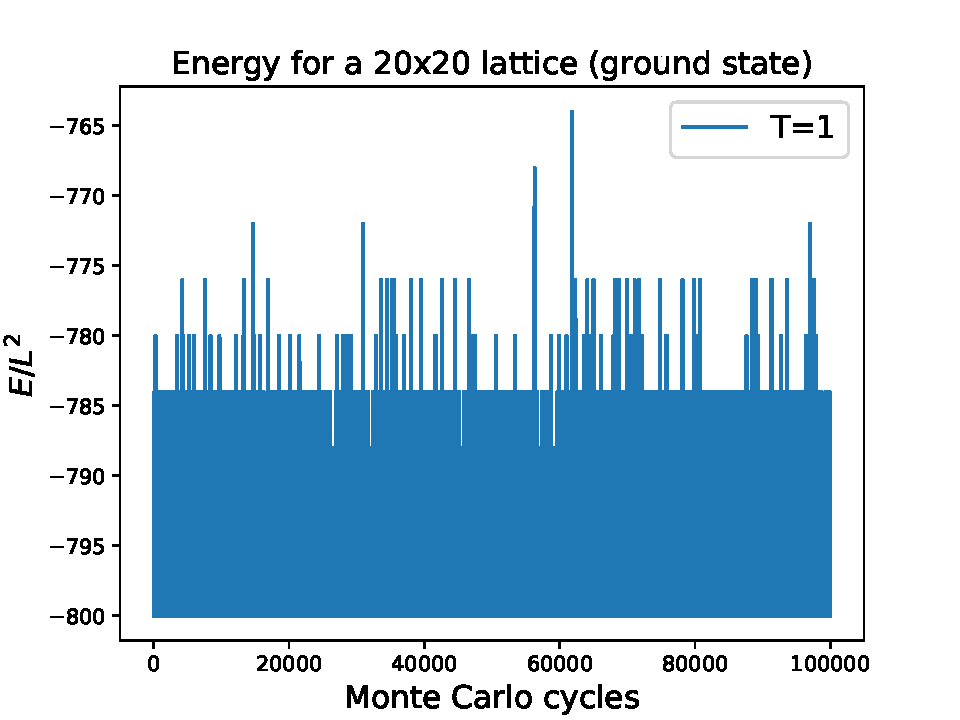
\includegraphics[width=9cm]{EofMCC-GS-T1-L20-1e5.pdf}
  \label{fig:L20-GS-E-T1}}\\
\subfloat[Absolute value of the magnetic moment pr. spin.]{
  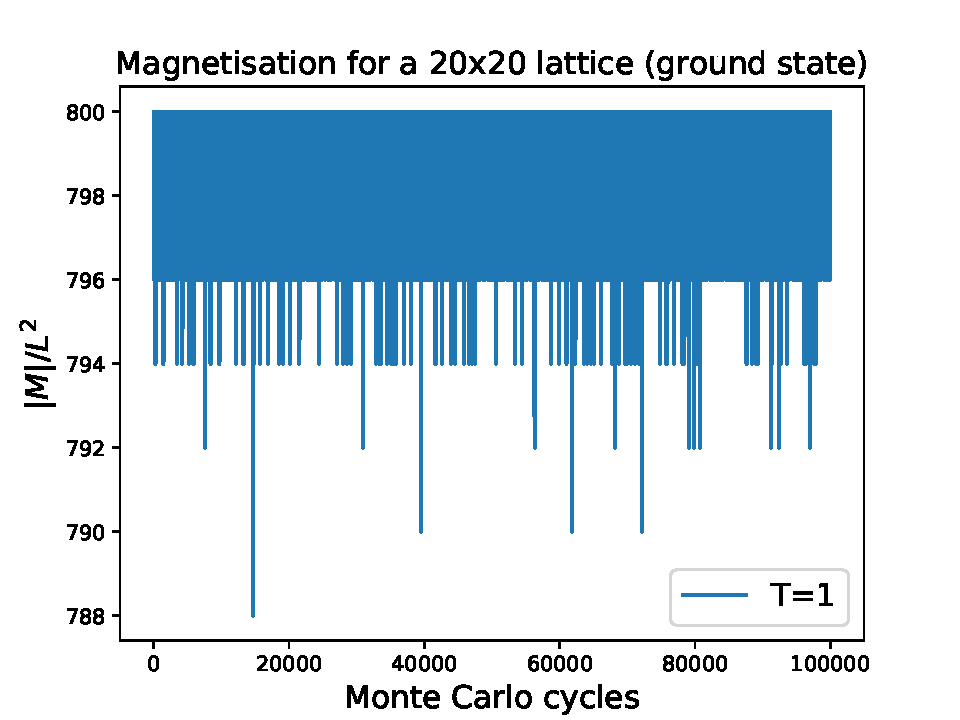
\includegraphics[width=9cm]{MofMCC-GS-T1-L20-1e5.pdf}
  \label{fig:evaluation:L20-GS-M-T1}}
\caption{Time evolution (MC cycles) of energy and magnetic moment of an ordered initial state with temperature 1 kT/J. $10^5$ Monte Carlo cycles.}
\end{figure}



\begin{figure}[h]
\subfloat[Energy pr. spin.]{%
  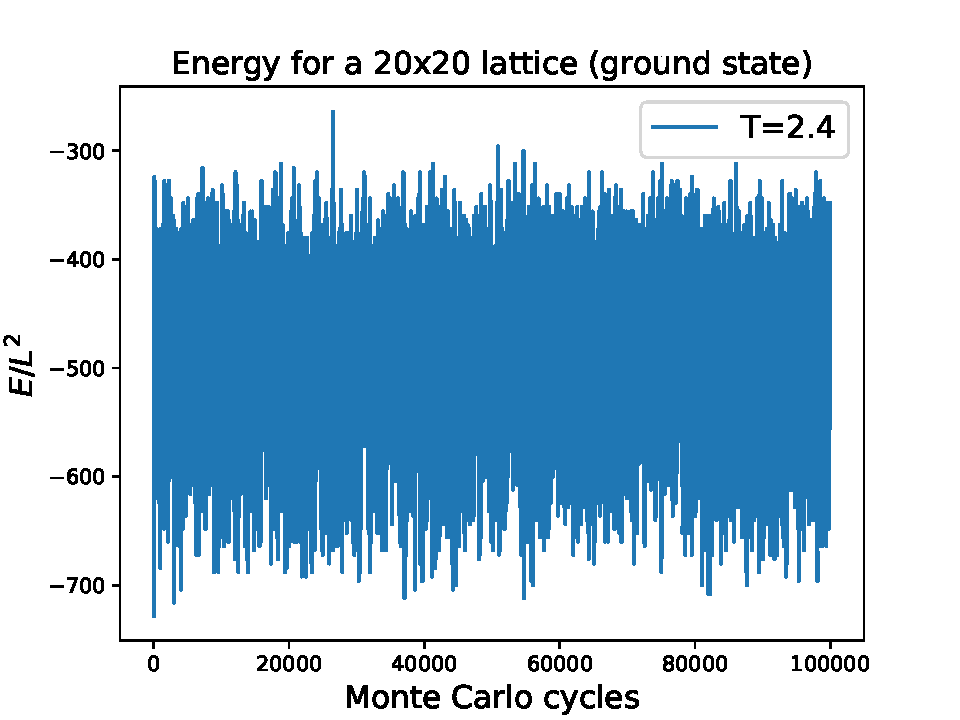
\includegraphics[width=8.65cm]{EofMCC-GS-T2_4-L20-1e5.pdf}
  \label{fig:L20-GS-E-T2.4}}\\
\subfloat[Absolute value of the magnetic moment pr. spin.]{
  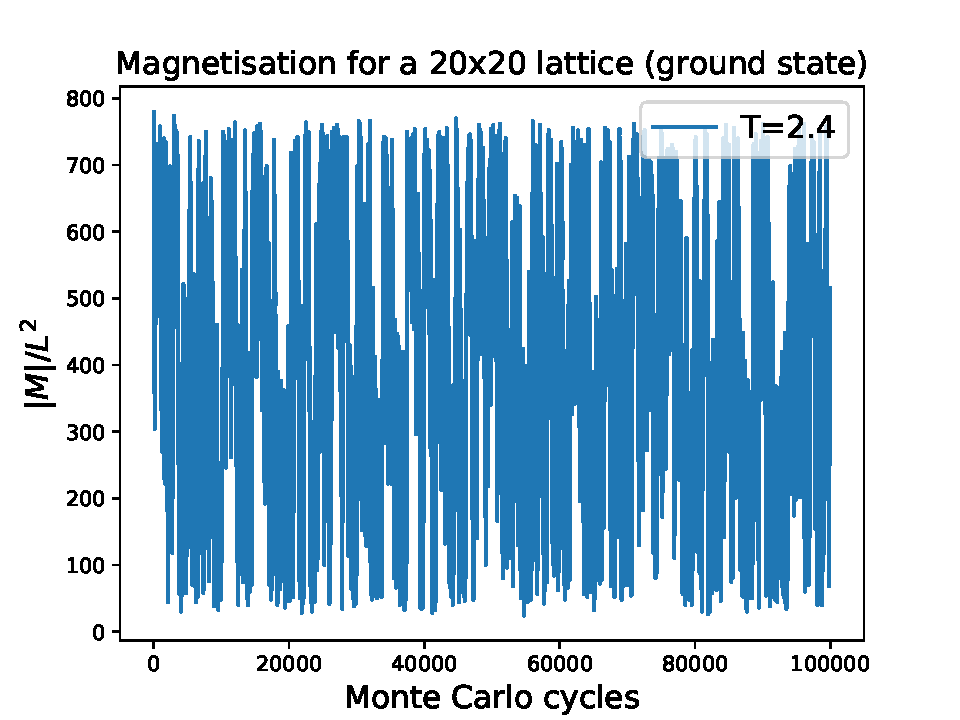
\includegraphics[width=8.65cm]{MofMCC-GS-T2_4-L20-1e5.pdf}
  \label{fig:L20-GS-M-T2.4}}
\caption{Time evolution of energy and magnetic moment of an ordered initial state with temperature 2.4 kT/J. $10^5$ Monte Carlo cycles.}
\end{figure}

\begin{figure}[h]
\subfloat[Energy pr. spin.]{%
  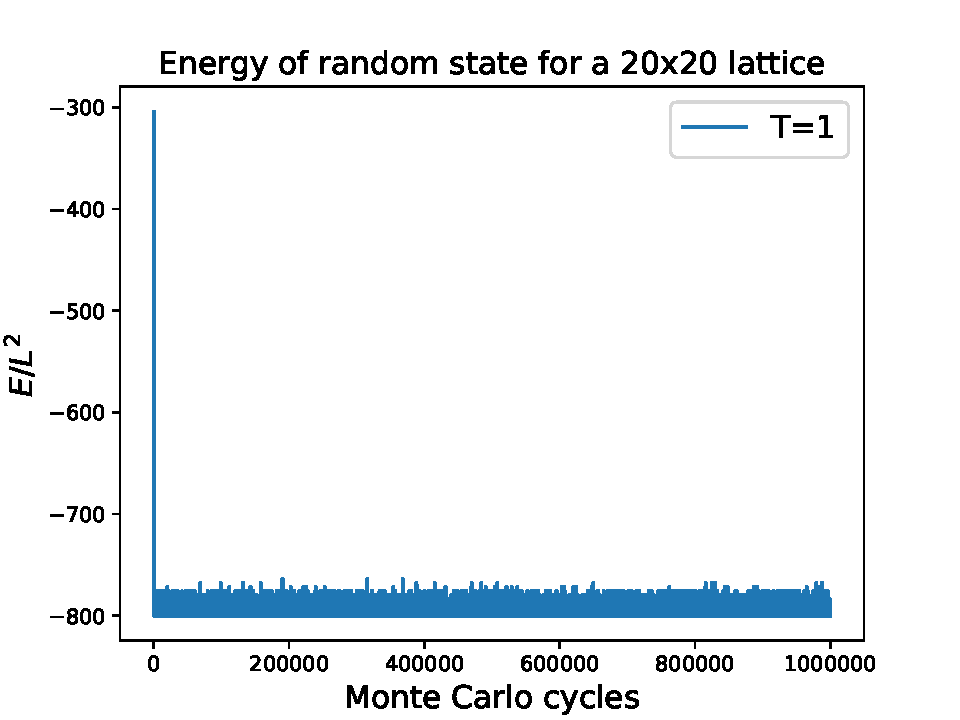
\includegraphics[width=8.65cm]{EofMCC-T1-L20-1e6.pdf}%
  \label{fig:L20-E-T1}%
}\\
\subfloat[Absolute value of the magnetic moment pr. spin.]{%
  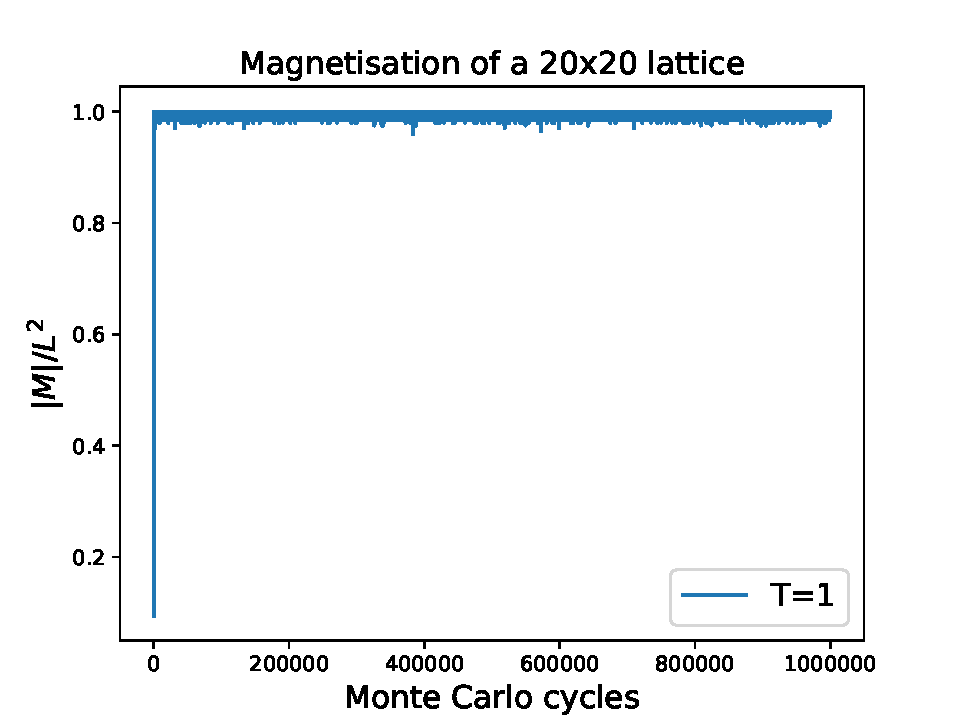
\includegraphics[width=8.65cm]{MofMCC-T1-L20-1e6.pdf}%
  \label{fig:L20-M-T1}%
}
\caption{Time evolution of energy and magnetic moment of an random initial state with temperature 1 kT/J. $10^6$ Monte Carlo cycles.}
\end{figure}

\begin{figure}[h]
\subfloat[Energy pr. spin.]{
  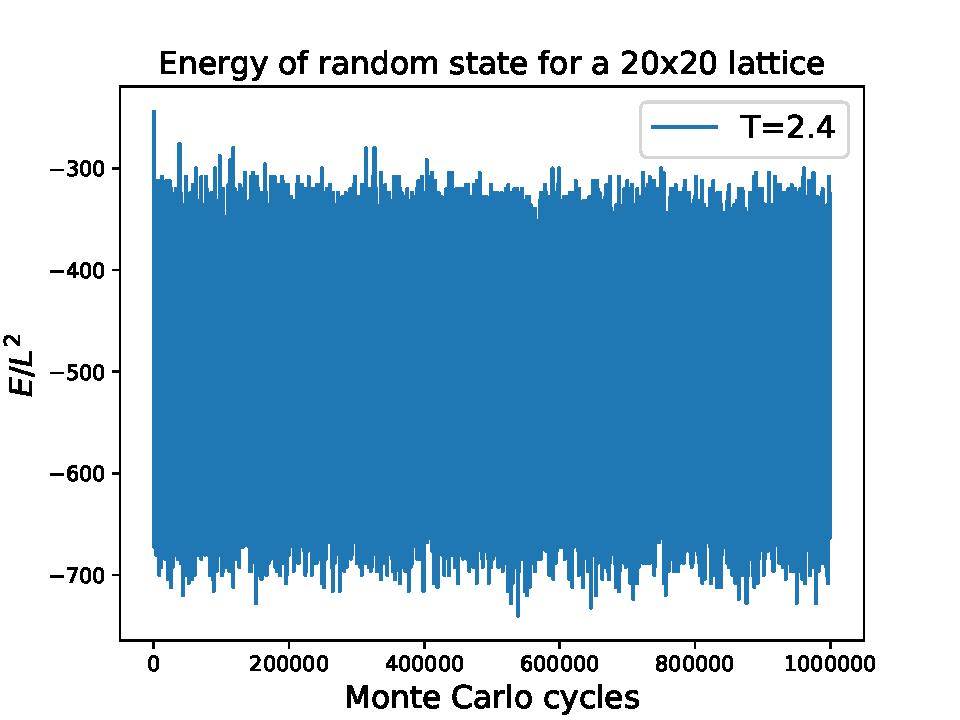
\includegraphics[width=8.65cm]{EofMCC-T2_4-L20-1e6.pdf}
  \label{fig:evaluation:revenue}}\\
\subfloat[Absolute value of the magnetic moment pr. spin.]{
  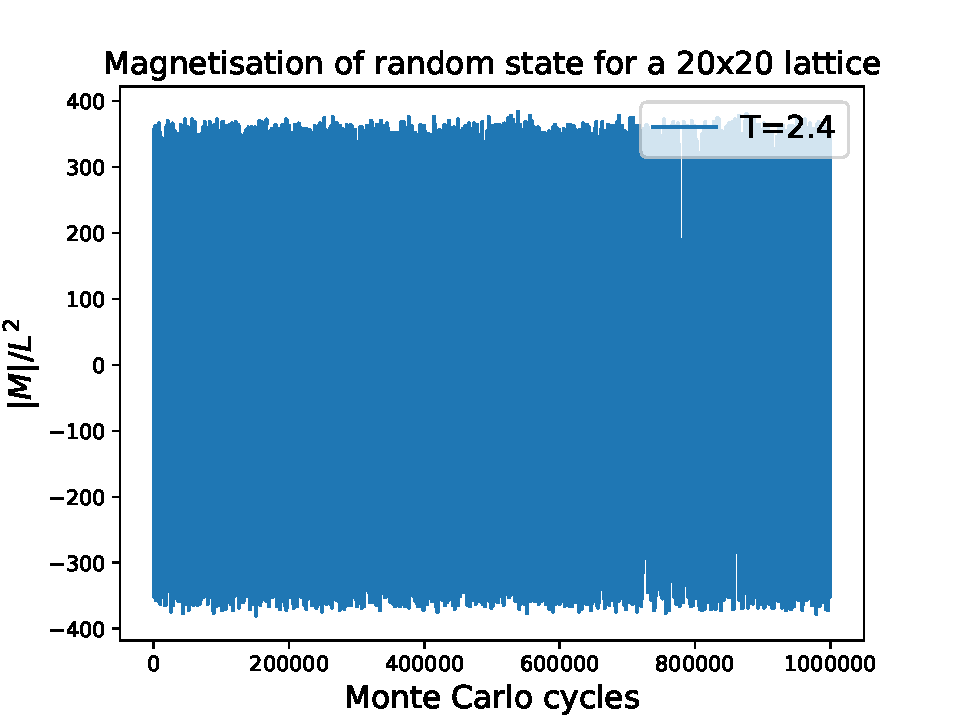
\includegraphics[width=8.65cm]{MofMCC-T2_4-L20-1e6.pdf}
  \label{fig:evaluation:avgPrice}}
\caption{Time evolution (MC cycles) of energy and magnetic moment of an random initial state with temperature 2.4 kT/J. $10^6$ Monte Carlo cycles.}
\end{figure}

\begin{figure}[h]
\mbox{\epsfig{figure=accepts_of_T-T1T2_4-L20.pdf,width=\linewidth,clip=}}
\caption{Logarithm of the accepted states as a function of the temperature for different number of Monte Carlo cycles. The left four dots corresponds to $T=1$ kT/J, and the right four dots corresponds to $T=2.4$ kT/J. The initial spins are randomly organized.}
\label{fig:logAccepts(t)}
\end{figure}

\begin{figure}[h]
\mbox{\epsfig{figure=accepts-T1T2_4-L20-1e5.pdf,width=\linewidth,clip=}}
\caption{Logarithmic plot of accepted states as a function of Monte Carlo cycles. The initial spins are randomly organized.}
\label{fig:logAccepts}
\end{figure}


\begin{figure}[h]
\mbox{\epsfig{figure=E-T2-23.pdf,width=\linewidth,clip=}}
\caption{Mean energy pr. spin for various amounts of MC cycles. Initial spin state is random. Temperature varies with a step size of 0.03, making it ten steps.}
\label{fig:E-T2-23}
\end{figure}

\begin{figure}[h]
\mbox{\epsfig{figure=M-T2-23.pdf,width=\linewidth,clip=}}
\caption{Mean absolute value of magnetic moment pr. spin for various amounts of MC cycles. Initial spin state is random. Temperature varies with a step size of 0.03, making it ten steps.}
\label{fig:M-T2-23}
\end{figure}

\begin{figure}[h]
\mbox{\epsfig{figure=CV-T2-23.pdf,width=\linewidth,clip=}}
\caption{Heat capacity pr. spin for various amounts of MC cycles. Initial spin state is random. Temperature varies with a step size of 0.03, making it ten steps.}
\label{fig:CV-T2-23}
\end{figure}

\begin{figure}[h]
\mbox{\epsfig{figure=X-T2-23.pdf,width=\linewidth,clip=}}
\caption{Susceptibility pr. spin for various amounts of MC cycles. Initial spin state is random. Temperature varies with a step size of 0.03, making it ten steps.}
\label{fig:chi-T2-23}
\end{figure}

\begin{figure}[h]
\mbox{\epsfig{figure=E-T22-24.pdf,width=\linewidth,clip=}}
\caption{Mean energy pr. spin for various amounts of MC cycles. Initial spin state is random. Temperature varies with a step size of 0.01, making it twenty steps.}
\label{fig:E-T22-23}
\end{figure}

\begin{figure}[h]
\mbox{\epsfig{figure=M-T22-24.pdf,width=\linewidth,clip=}}
\caption{Mean abslute value of the magnetic moment pr. spin for various amounts of MC cycles. Initial spin state is random. Temperature varies with a step size of 0.01, making it twenty steps.}
\label{fig:M-T22-23}
\end{figure}

\begin{figure}[h]
\mbox{\epsfig{figure=CV-T22-24.pdf,width=\linewidth,clip=}}
\caption{Heat capacity pr. spin for various amounts of MC cycles. Initial spin state is random. Temperature varies with a step size of 0.01, making it twenty steps.}
\label{fig:CV-T22-24}
\end{figure}

\begin{figure}[h]
\mbox{\epsfig{figure=X-T22-24.pdf,width=\linewidth,clip=}}
\caption{Susceptibility pr. spin for various amounts of MC cycles. Initial spin state is random. Temperature varies with a step size of 0.01, making it twenty steps.}
\label{fig:chi-T22-23}
\end{figure}

\begin{figure}[h]
\mbox{\epsfig{figure=FittedTc.pdf,width=\linewidth,clip=}}
\caption{Linear regression used on the critical temperatures at points of 1/L for $L = 40$, $60$, $80$ and $100$ gives the function $y(x) = 3.45x + 2.22$.}
\label{fig:figure_label}
\end{figure}


\begin{figure}[h]
\mbox{\epsfig{figure=PE-T1-L20-1e6.pdf,width=\linewidth,clip=}}
\caption{Histogram of the probability as a function of energy. Temperature is 1 kT/J. Initial spin states are random.}
\label{fig:figure_label}
\end{figure}


\begin{figure}[h]
\mbox{\epsfig{figure=PE-T2_4-L20-1e6.pdf,width=\linewidth,clip=}}
\caption{Histogram of the probability as a function of energy. Temperature is 2.4 kT/J. Initial spin states are random.}
\label{fig:figure_label}
\end{figure}

\begin{deluxetable}{cccc}
\tablewidth{0pt}
\tablecaption{\label{tab:runtimes40}}
\tablecomments{Run times for a 40x40 lattice for $10^5$ Monte Carlo cycles. Temperature set to 1 kT/J and the initial state for the spins are random.}
\tablecolumns{4}
\tablehead{Run & 1 core & 4 core & Difference}
\startdata
1 & 13.910 & 4.448 & 9.461 \\
2 & 14.348 & 4.530 & 9.817 \\
3 & 14.407 & 4.636 & 9.770 \\
Average & 14.221 & 4.538 & 9.683
\enddata
\end{deluxetable}

\begin{deluxetable}{cccc}
\tablewidth{0pt}
\tablecaption{\label{tab:runtimes100}}
\tablecomments{Run times for a 100x100 lattice for $10^5$ Monte Carlo cycles. Temperature set to 1 kT/J and the initial state for the spins are random.}
\tablecolumns{5}
\tablehead{Run & 1 core & 4 core & Difference}
\startdata
1 & 91.137 & 34.434 & 62.702 \\
2 & 83.662 & 30.455 & 53.207 \\
3 & 86.905 & 28.534 & 58.371 \\
Average & 87.235 & 31.141 & 58.093
\enddata
\end{deluxetable}






\section{Discussion}
\label{sec:discussion}




\section{Conclusions}
\label{sec:conclusions}




%\begin{figure}[h]
%
%\mbox{\epsfig{figure=filename.eps,width=\linewidth,clip=}}
%
%\caption{Description of figure -- explain all elements, but do not
%draw conclusions here.}
%\label{fig:figure_label}
%\end{figure}



%\begin{deluxetable}{lccc}
%\tablewidth{0pt}
%\tablecaption{\label{tab:results}}
%\tablecomments{Summary of main results.}
%\tablecolumns{4}
%\tablehead{Column 1  & Column 2 & Column 3 & Column 4}
%\startdata
%Item 1 & Item 2 & Item 3 & Item 4
%\enddata
%\end{deluxetable}



\begin{acknowledgements}

\end{acknowledgements}

\begin{thebibliography}{}

\bibitem[G{\'o}rski et al.(1994)]{gorski:1994} G{\'o}rski, K. M.,
  Hinshaw, G., Banday, A. J., Bennett, C. L., Wright, E. L., Kogut,
  A., Smoot, G. F., and Lubin, P.\ 1994, ApJL, 430, 89

\end{thebibliography}


\end{document}
